\documentclass[spanish, 10pt]{article}

\usepackage[table, xcdraw]{xcolor}
\usepackage[utf8]{inputenc}
\usepackage[spanish, mexico]{babel}
\usepackage{helvet}
\usepackage{fullpage}
\usepackage{graphicx}
\usepackage{enumitem}
\usepackage{tikz}
\usepackage{ulem}
\usepackage{url}
\usepackage{hyperref}
\usepackage[margin = 3 cm]{geometry}
\usepackage{amsmath}
\usepackage{amsfonts}

\usepackage{matlab-prettifier}
\usepackage{multicol}

\usetikzlibrary{arrows, shapes, trees, calc, decorations.pathreplacing, shapes.misc, positioning, automata}

\setlength\parindent{0pt}

\renewcommand{\familydefault}{\sfdefault}
\newcommand{\responserule}{{\large\rule{14 cm}{0.3mm}}}
\newcommand{\shortresponserule}{{\large\rule{5 cm}{0.3mm}}}
\newcommand{\veryshortresponserule}{{\large\rule{3 cm}{0.3mm}}}
\newcommand{\matlab}[1]{\lstinline[style=Matlab-pyglike]!#1!}


% Specifications for listing package
% \lstset{	
%     basicstyle = \scriptsize\ttfamily,
%     keywordstyle = \color{blue}\ttfamily,
%     stringstyle = \color{red}\ttfamily,
%    	commentstyle = \color{gray}\ttfamily,
%    	tabsize = 3,
%    	breaklines = true,
%    	stepnumber = 1,
%    	showtabs = false,
%    	showstringspaces = false,
%    	frame = none
% }

% Commands for true/false questions
% ----------------------------------------------------------------
\newcommand{\question}[1]{%
	\noindent
	\begin{minipage}[t]{0.15\linewidth}
	\centering		
		\textbf{[\hspace{1 cm}]}
	\end{minipage}%
	\begin{minipage}[t]{0.85\linewidth}
		#1
	\end{minipage}
	\smallskip
}
% ----------------------------------------------------------------

\setlength\parindent{0pt}

\begin{document}

\begin{center}
	{\Large \textbf{Modelación de la Ingeniería con Matemática Computacional (TC-1003B)}}
	
	\bigskip
	{\large \textbf{Actividad 04 -- Aplicación de álgebra matricial}}
\end{center}

\bigskip
{\large \textbf{Nombre}: \rule{13.7 cm}{0.4mm}}

% \bigskip
% {\large \textbf{Matrícula}: \rule{5 cm}{0.4mm}}

% \bigskip
% {\large \textbf{Name}: \rule{14 cm}{0.4mm}}

\bigskip
{\large \textbf{Matrícula}: \rule{5 cm}{0.4mm}} \hfill {\large \textbf{Fecha}: \today}

\bigskip

% {\footnotesize Nota: es probable que esta actividad nos asuste un poco al principio. Es perfectamente normal.
% En efecto, es de mayor dificultad a las que hemos visto anteriormente y probablemente haya dudas.
% Si hay algo que no entiendas, no te quedes sin preguntar.}

\section{Matrices}

Para el siguiente grafo $G$

\begin{figure}[htbp]
    \centering
    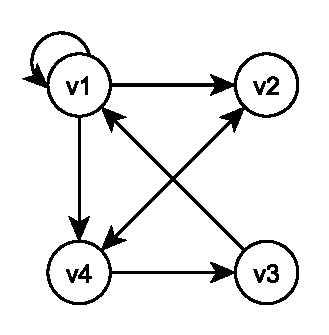
\includegraphics{digraph02.pdf}
    \caption{Grafo dirigido $G$}
    \label{fig:digraph}
\end{figure}

\begin{enumerate}
    \item ¿Cuáles son las dimensiones de la matriz de adyacencia $A$ del grafo $G$? \hfill \veryshortresponserule
    \item ¿Cuáles son los posibles valores que puede tener cada casilla de la matriz? \hfill \veryshortresponserule
    \item Si yo sumara todos los valores de una fila, ¿Cuál es el valor mínimo que obtendría y por qué? \\[2ex]\responserule
    \item Si yo sumara todos los valores de una fila, ¿Cuál es el valor máximo que obtendría y por qué? \\[2ex]
    \responserule
\end{enumerate}

Escribe la matriz de adyacencia $A$ a continuación:

\vspace{20ex}

\begin{itemize}
    \item ¿Cuántos caminos de longitud 2 hay entre $v2$ y $v3$? \hfill \veryshortresponserule
    \item ¿Cuántos caminos de longitud 3 hay entre $v1$ y $v4$? \hfill \veryshortresponserule
    \item ¿Cuántos caminos de longitud 3 hay entre $v2$ y $v3$? \hfill \veryshortresponserule
\end{itemize}

Justifica tu respuesta haciendo las multiplicaciones pertinentes.

\vspace{65ex}

\section{Reflexión}

Escribe los conceptos, tips o símbolos que consideres útiles para recordar lo visto en la sesión. Esta hoja te será de utilidad durante el examen.

\vfill

\textbf{Apegándome al Código de Ética de los Estudiantes del Tecnológico de Monterrey, me comprometo a que mi actuación en esta actividad esté regida por la honestidad académica.}

\end{document}